\documentclass[border=10pt]{standalone}
\usepackage[utf8]{inputenc}
\usepackage[T1]{fontenc}
\usepackage{tikz}
\usetikzlibrary{shapes.geometric, arrows.meta, positioning, fit, backgrounds, shadows}

\begin{document}

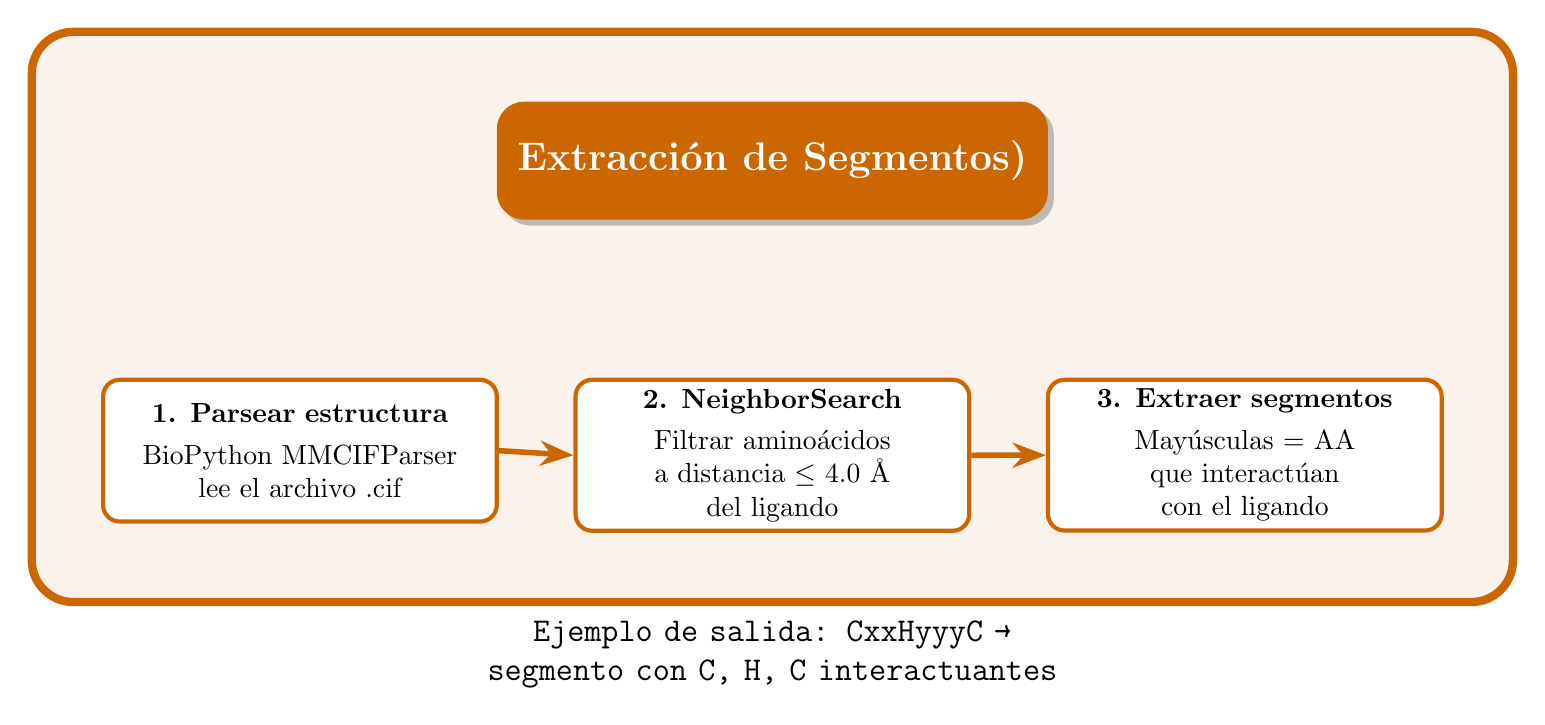
\begin{tikzpicture}[
        node distance=1.5cm,
        % Estilos para nodos principales
        mainbox/.style={
                rectangle,
                rounded corners=10pt,
                minimum width=7cm,
                minimum height=1.5cm,
                text centered,
                text width=6.5cm,
                font=\bfseries\Large,
                text=white,
                drop shadow
            },
        % Estilos para sub-nodos
        subbox/.style={
                rectangle,
                rounded corners=6pt,
                minimum width=5cm,
                minimum height=1.8cm,
                text centered,
                text width=4.5cm,
                font=\normalsize,
                text=black,
                fill=white,
                draw=orange!80!black,
                line width=1.5pt
            },
        % Flechas
        arrow/.style={
                ->,
                >=Stealth,
                line width=2pt,
                color=orange!80!black
            },
        % Grupo contenedor
        groupbox/.style={
                rectangle,
                rounded corners=15pt,
                draw=orange!80!black,
                line width=3pt,
                fill=orange!80!black!8,
                inner sep=25pt
            }
    ]

    % Título principal
    \node[mainbox, fill=orange!80!black] (extraccion) {Extracción de Segmentos)};

    % Sub-nodos
    \node[subbox, below=2cm of extraccion, xshift=-6cm] (ext1) {
        \textbf{1. Parsear estructura}\\[3pt]
        BioPython MMCIFParser\\
        lee el archivo .cif
    };

    \node[subbox, below=2cm of extraccion] (ext2) {
        \textbf{2. NeighborSearch}\\[3pt]
        Filtrar aminoácidos\\
        a distancia $\leq$ 4.0 Å\\
        del ligando
    };

    \node[subbox, below=2cm of extraccion, xshift=6cm] (ext3) {
        \textbf{3. Extraer segmentos}\\[3pt]
        Mayúsculas = AA\\
        que interactúan\\
        con el ligando
    };

    % Grupo
    \begin{scope}[on background layer]
        \node[groupbox, fit=(extraccion)(ext1)(ext2)(ext3)] (gext) {};
    \end{scope}

    % Flechas entre sub-nodos
    \draw[arrow] (ext1.east) -- (ext2.west);
    \draw[arrow] (ext2.east) -- (ext3.west);

    % Ejemplo
    \node[below=1cm of ext2, text width=12cm, align=center, font=\ttfamily\large] (ejemplo) {
        Ejemplo de salida: \textbf{CxxHyyyC} → segmento con C, H, C interactuantes
    };

\end{tikzpicture}

\end{document}
